\documentclass[a4paper,11pt]{article}

\usepackage[T1]{fontenc}
\usepackage[utf8]{inputenc}
\usepackage{graphicx}
\usepackage{xcolor}

\renewcommand\familydefault{\sfdefault}
\usepackage{tgheros}
\usepackage[defaultmono]{droidmono}

\usepackage{amsmath,amssymb,amsthm,textcomp}
\usepackage{enumerate}
\usepackage{multicol}
\usepackage{tikz}


\graphicspath{ {.} }
\usepackage{geometry}
\geometry{left=25mm,right=25mm,%
bindingoffset=0mm, top=20mm,bottom=20mm}


\linespread{1.3}

\newcommand{\linia}{\rule{\linewidth}{0.5pt}}

% custom theorems if needed
\newtheoremstyle{mytheor}
    {1ex}{1ex}{\normalfont}{0pt}{\scshape}{.}{1ex}
    {{\thmname{#1 }}{\thmnumber{#2}}{\thmnote{ (#3)}}}

\theoremstyle{mytheor}
\newtheorem{defi}{Definition}

% my own titles
\makeatletter
\renewcommand{\maketitle}{
\begin{center}
\vspace{2ex}
{\huge \textsc{\@title}}
\vspace{1ex}
\\
\linia\\
\@author \hspace{100ex} BS18-02 \hspace{100ex} Variant (k)

\vspace{4ex}
\end{center}
}
\makeatother
%%%

% custom footers and headers
\usepackage{fancyhdr}
\pagestyle{fancy}
\lhead{}
\chead{}
\rhead{}
\lfoot{Assignment \textnumero{} 1}
\cfoot{}
\rfoot{Page \thepage}
\renewcommand{\headrulewidth}{0pt}
\renewcommand{\footrulewidth}{0pt}
%

% code listing settings
\usepackage{listings}
\lstset{
    language=Python,
    basicstyle=\ttfamily\small,
    aboveskip={1.0\baselineskip},
    belowskip={1.0\baselineskip},
    columns=fixed,
    extendedchars=true,
    breaklines=true,
    tabsize=4,
    prebreak=\raisebox{0ex}[0ex][0ex]{\ensuremath{\hookleftarrow}},
    frame=lines,
    showtabs=false,
    showspaces=false,
    showstringspaces=false,
    keywordstyle=\color[rgb]{0.627,0.126,0.941},
    commentstyle=\color[rgb]{0.133,0.545,0.133},
    stringstyle=\color[rgb]{01,0,0},
    numbers=left,
    numberstyle=\small,
    stepnumber=1,
    numbersep=10pt,
    captionpos=t,
    escapeinside={\%*}{*)}
}

%%%----------%%%----------%%%----------%%%----------%%%

\begin{document}

\title{HW \textnumero{} 1}

\author{Matvey Plevako}

\maketitle


\section*{Problem 1}


$x''= x' - 5 x-3 \sin{t}$ \\
$x'(0)=0,x(0)=-5$


\section*{Part A}

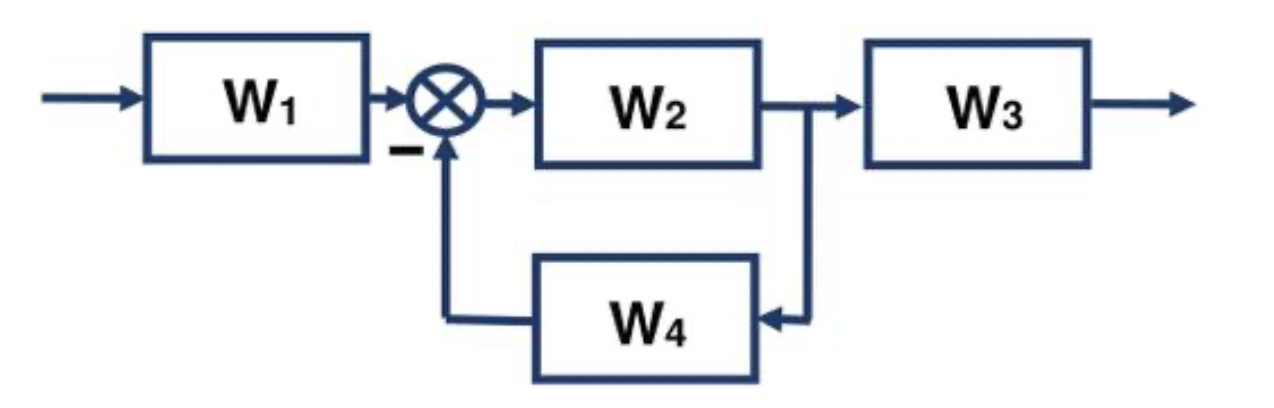
\includegraphics[width=15.3cm, height=6cm]{1.png}

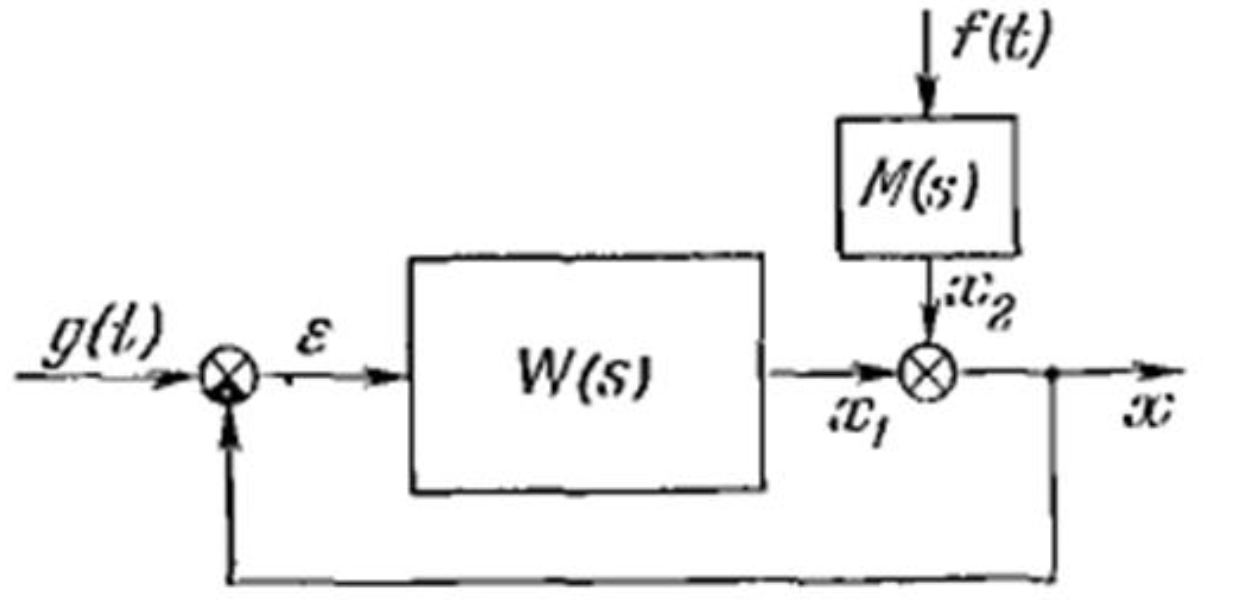
\includegraphics[width=8cm, height=6cm]{2.png}


\section*{Part B}
Calculations of transfer function. \\
$\frac{\partial}{\partial t} = p$ \\
$p^2x - px +5x + 3\sin{t} = 0$ \\
$(p^2 - p + 5)x = -3\sin{t}$ \\
$x = \frac{1}{p^2 - p + 5} * (-3\sin{t})$

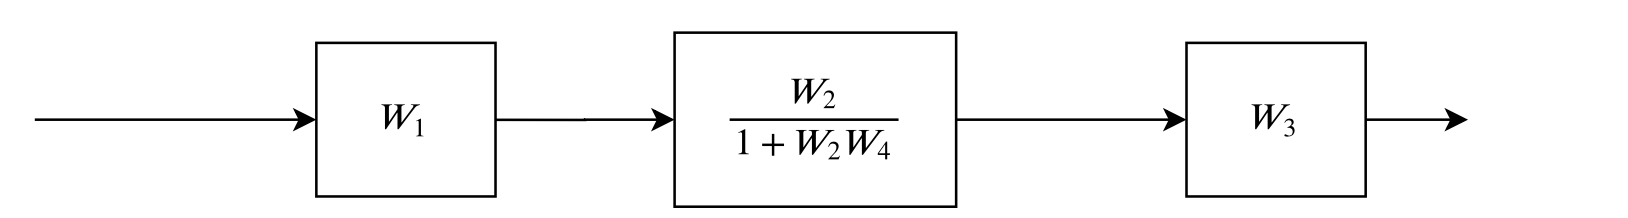
\includegraphics[width=14cm, height=4cm]{3.png}

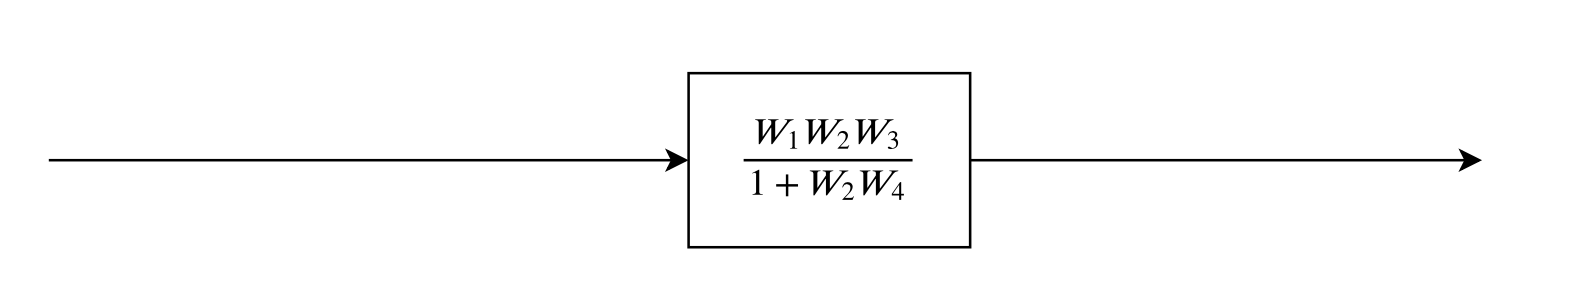
\includegraphics[width=8cm, height=6cm]{4.png}

\section*{Part C}
Code for solving differential equation
\begin{lstlisting}
>> syms x(t)
>> Dx = diff(x,t);
>> eqn = diff(x,t,2) == Dx - 5 * x - 3 * sin(t);
>> cond = [x(0)==-5, Dx(0)==0];
>> xSol(t) = dsolve(eqn,cond)
 
xSol(t) =
 
- (82*exp(t/2)*cos((19^(1/2)*t)/2))/17 - cos((19^(1/2)*t)/2)*((3*cos(t - (19^(1/2)*t)/2))/34 + (3*cos(t + (19^(1/2)*t)/2))/34 + (6*sin(t - (19^(1/2)*t)/2))/17 + (6*sin(t + (19^(1/2)*t)/2))/17 + (9*19^(1/2)*cos(t - (19^(1/2)*t)/2))/323 - (9*19^(1/2)*cos(t + (19^(1/2)*t)/2))/323 + (21*19^(1/2)*sin(t - (19^(1/2)*t)/2))/646 - (21*19^(1/2)*sin(t + (19^(1/2)*t)/2))/646) - (3*19^(1/2)*sin((19^(1/2)*t)/2)*((sin(t*(19^(1/2)/2 - 1))/2 + cos(t*(19^(1/2)/2 - 1))*(19^(1/2)/2 - 1))/((19^(1/2)/2 - 1)^2 + 1/4) - (sin(t*(19^(1/2)/2 + 1))/2 + cos(t*(19^(1/2)/2 + 1))*(19^(1/2)/2 + 1))/((19^(1/2)/2 + 1)^2 + 1/4)))/19 - (106*19^(1/2)*exp(t/2)*sin((19^(1/2)*t)/2))/(19*(19^(1/2) - 6)*(19^(1/2) + 6))
 
>> 
>> fplot(xSol)

\end{lstlisting}

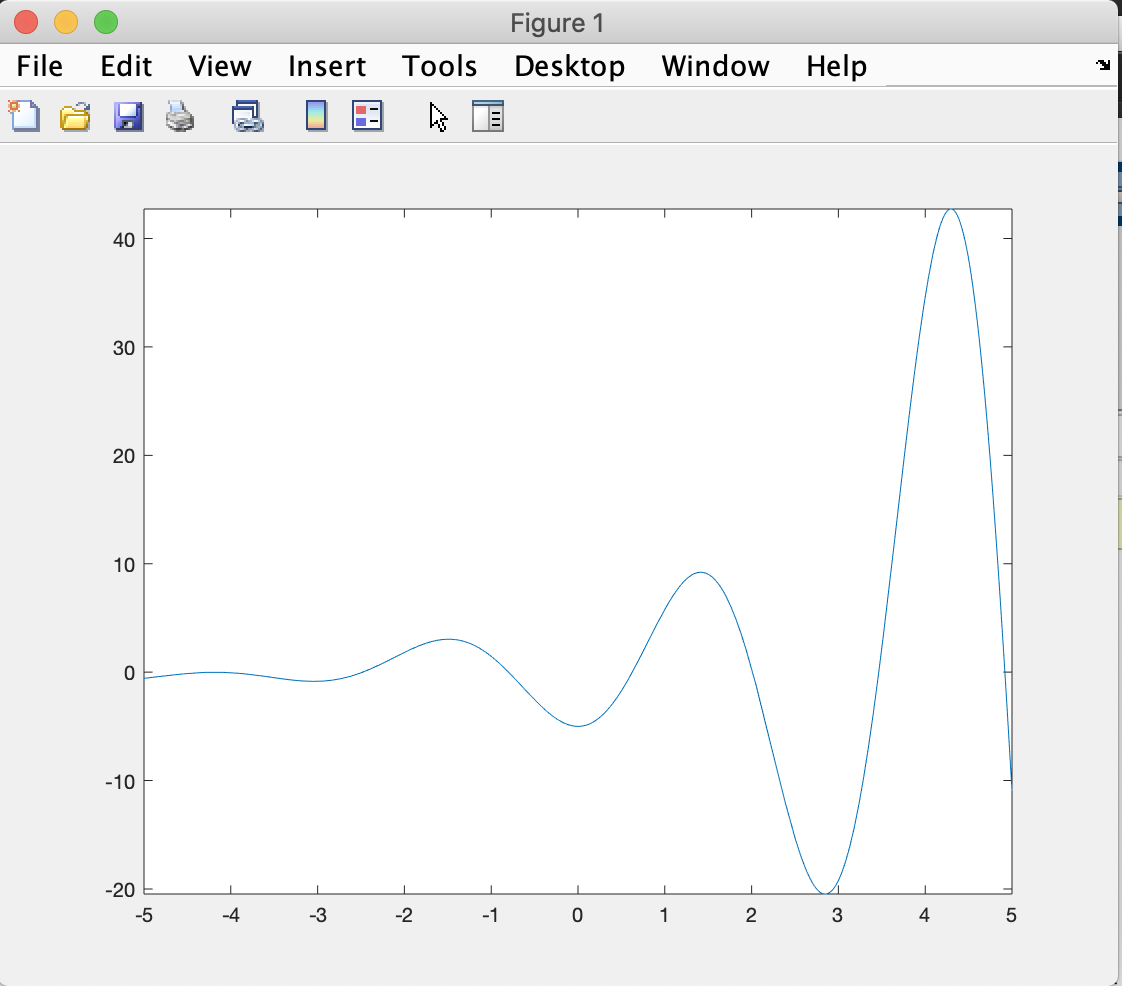
\includegraphics[width=8cm, height=6cm]{5.png}

\section*{Part D}
Code for solving differential equation with Laplace 
\begin{lstlisting}
>> syms x t s
>> f = -3 * sin(t)
 
f =
 
-3*sin(t)
 
>> F = laplace(f, t, s)
 
F =
 
-3/(s^2 + 1)
 
>> X1 = s * x + 5
 
X1 =
 
s*x + 5
 
>> X2 = s * X1
 
X2 =
 
s*(s*x + 5)
 
>> Sol = solve(X2 - X1 + 5 * x + 3 * sin(t), x)
 
Sol =
 
-(5*s + 3*sin(t) - 5)/(s^2 - s + 5)
 
>> sol = ilaplace(Sol,s,t)
 
sol =
 
-5*exp(t/2)*(cos((19^(1/2)*t)/2) + (2*19^(1/2)*sin((19^(1/2)*t)/2)*((3*sin(t))/5 - 1/2))/19)
 
>> fplot(sol)
\end{lstlisting}

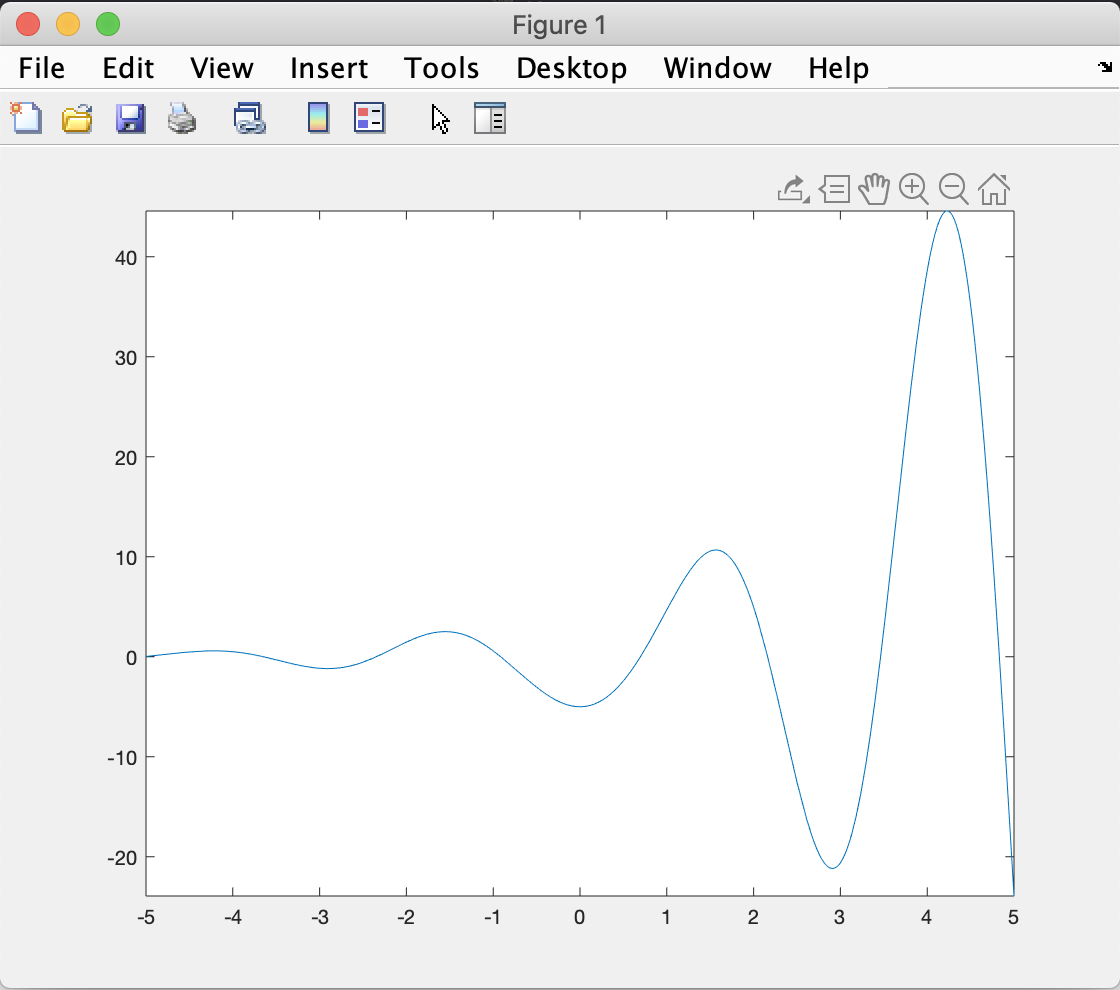
\includegraphics[width=8cm, height=6cm]{6.png}

\section*{Problem 2}

\begin{equation}
\begin{cases}
    x''-x'+5=t+1 \\ y = 2x + x'
\end{cases}
\end{equation}

$x''=x'+t-4$ 

$ \begin{bmatrix}x'\\x''\end{bmatrix} = \begin{bmatrix}0&1\\0&1\end{bmatrix} * \begin{bmatrix}x\\x'\end{bmatrix} + \begin{bmatrix}0\\1\end{bmatrix} * (t-4)$

$ \begin{bmatrix}y\end{bmatrix} = \begin{bmatrix}2&1\end{bmatrix} * \begin{bmatrix}x\\x'\end{bmatrix} + \begin{bmatrix}0\end{bmatrix} * u$

\section*{Problem 3}

\begin{equation}
\begin{cases}
    x'''' - x''' - x'' +3x' +x = 3u_1 +u_2 \\ y=x' +u_1
\end{cases}
\end{equation}

$x'''' = x''' + x'' - 3x' - x + 3u_1 + u_2 $

$ \begin{bmatrix}x'\\x''\\x'''\\x''''\end{bmatrix} = \begin{bmatrix}0&1&0&0\\0&0&1&0\\0&0&0&1\\-1&-3&1&1\end{bmatrix} * \begin{bmatrix}x\\x'\\x''\\x'''\end{bmatrix}  + \begin{bmatrix}0&0\\0&0\\0&0\\3&1\end{bmatrix} * \begin{bmatrix}u_1\\u_2\end{bmatrix}$

$ \begin{bmatrix}y\end{bmatrix} = \begin{bmatrix}0&1&0&0\end{bmatrix} * \begin{bmatrix}x\\x'\\x''\\x'''\end{bmatrix} + \begin{bmatrix}1&0\end{bmatrix} * \begin{bmatrix}u_1\\u_2\end{bmatrix}$

\section*{Problem 4}

% code from http://rosettacode.org/wiki/Fibonacci_sequence#Python
\begin{lstlisting}[label={list:first}]
import numpy as np

# return matrix A and b
# 1. divide by a_k 
# 2. express y^(k) derivative 
# 3. create matrix and replace the last row with reverse coefficients
def convert_ODE_to_SS(coefs, b0):
  b0 /= coefs[0]
  coefs = coefs / coefs[0]
  A = np.eye(len(coefs), k=1)
  A[-1] = coefs[::-1]
  B = np.zeros((3, 1))
  B[-1][0] = b0
  return A, B
  
  
coef = np.array([3, 2, 1])
convert_ODE_to_SS(coef, 3)

(array([[0.        , 1.        , 0.        ],
        [0.        , 0.        , 1.        ],
        [0.33333333, 0.66666667, 1.        ]]), array([[0.        ],
        [0.        ],
        [0.33333333]]))
\end{lstlisting}


\section*{Problem 5}

\begin{lstlisting}[label={list:second}]

def pend(y, t, coefs, u):
  '''
  y: np array of shape (N) in order x(0), x'(0), x''(0) ...
  t: range
  coefs: np array of shape (N) in order a1*x, a2*x', a3*x'' ...
  u: function of t
  '''
  dydt = np.append(y[1:], coefs.dot(y) + u(t)) 
  return dydt


from scipy.integrate import odeint
from math import sin

coefs = np.array([-5, 1])
y0 = np.array([-5, 0])
u = lambda t: -3 * sin(t)
t = np.linspace(0, 10, 101)
sol = odeint(pend, y0, t, args=(coefs, u))



import matplotlib.pyplot as plt

plt.plot(t, sol[:, 0], 'b', label='x(t)')
plt.legend(loc='best')
plt.xlabel('t')
plt.grid()
plt.show()

\end{lstlisting}

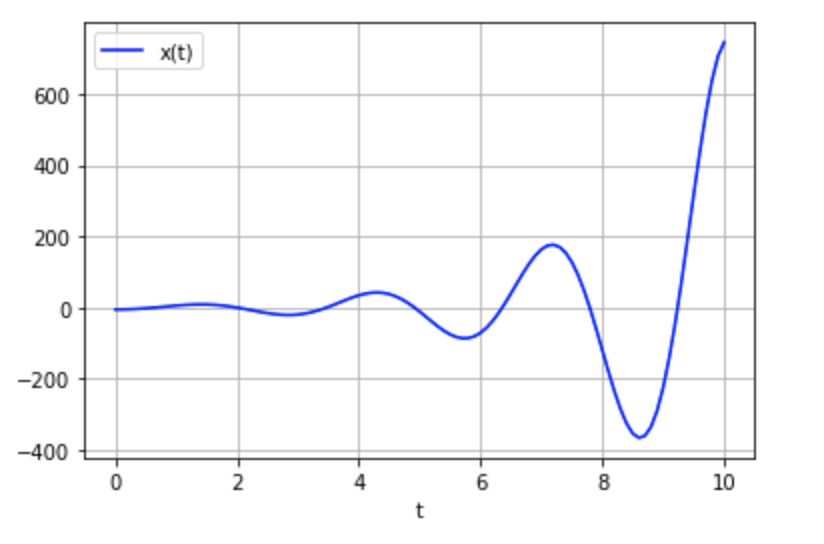
\includegraphics[width=8cm, height=6cm]{7.png}

\end{document}

